\documentclass[11pt,a4paper,xcolor=table]{beamer} % ,handout: for printing
\usepackage{etex}
%\documentclass[handout]{beamer}

%\usetheme{Madrid}

%
% To use when printing
%
\iffalse
\usepackage{pgfpages}
\mode<handout>{
  \usetheme{default}
  \setbeamercolor{}{bg=black!5} % \setbeamercolor{background canvas}{bg=black!5} 
  \pgfpagesuselayout{4 on 1}[letterpaper,landscape,border shrink=2.5mm]
}
\fi

\usepackage[utf8]{inputenc} % [utf8] for linux, latin1 for windows
\usepackage[french]{babel}
%\usepackage{fullpage}
\usepackage{amsmath}
\usepackage{amsfonts}
\usepackage{amssymb}
\usepackage{graphicx} 
\usepackage{longtable}
\usepackage{algorithm}
\usepackage{listings}
\usepackage{algorithmic}
\usepackage{float}

\usepackage[center]{caption}
\usepackage{subcaption}

\usepackage[table]{xcolor}

\definecolor{colorperso}{RGB}{165,165,165}
%\usepackage[utf8]{inputenc}
%\usepackage[francais]{babel}
%\usepackage[T1]{fontenc}

%\usepackage{amsmath}
%\usepackage{amsfonts}
%\usepackage{amssymb}

%\usepackage{amsthm}
%\usepackage{graphicx}

\usepackage{tikz,pgfplots}
\usepackage[all]{xy}

% tikz stuff
\usetikzlibrary{shapes,arrows,decorations.pathreplacing, calc, intersections}
\makeatletter
\newcommand{\gettikzxy}[3]{%
  \tikz@scan@one@point\pgfutil@firstofone#1\relax
  \edef#2{\the\pgf@x}%
  \edef#3{\the\pgf@y}%
}
\makeatother

\newtheorem*{mydef}{Definition}
%\newtheorem*{definition}{Definition}
\newtheorem{mythm}{Theorem}
\newtheorem{requirement}{Requirement}
\newtheorem*{mynot}{Notation}
\newtheorem{myprop}{Proposition}

\newcommand{\var}{\operatorname{Var}}


\makeatother
\setbeamertemplate{footline}
{
  \leavevmode%
  \hbox{%
  \begin{beamercolorbox}[wd=.4\paperwidth,ht=2.25ex,dp=1ex,center]{author in head/foot}%
    \usebeamerfont{author in head/foot}\insertshortauthor
  \end{beamercolorbox}%
  \begin{beamercolorbox}[wd=.6\paperwidth,ht=2.25ex,dp=1ex,center]{title in head/foot}%
    \usebeamerfont{title in head/foot}\insertshorttitle\hspace*{3em}
    \insertframenumber{} / \inserttotalframenumber\hspace*{1ex}
  \end{beamercolorbox}}%
  \vskip0pt%
}
\makeatletter

\setbeamertemplate{navigation symbols}{}

\author[]{Jean-Baptiste Lespiau}
\author{Jean-Baptiste Lespiau et Charles Thin}
\title{La méthode B : une méthode formelle de développement logiciel}
\date\today

\begin{document}

\frame{\titlepage}

\section*{Introduction}

\begin{frame}
\frametitle{Introduction}
%\framesubtitle{DTA overview}
La méthode B c'est langage unique permettant de :
\begin{itemize}
\item Spécifier
\item Raffiner ces spécifications
\item Aboutir à une implémentation
\end{itemize}

\pause
~\newline
L'Atelier B (ClearSy) permet d'encadrer le processus industriel :
\begin{itemize}
\item un analyseur~;
\item un générateur d'obligation de preuve~;
\item un démonstrateur automatique~;
\item un démonstrateur interactif~;
\item un générateur de code C et Ada~;
\item un gestionnaire de projet...
\end{itemize}
\end{frame}

\begin{frame}
\frametitle{Cycle de développement formel vs cycle conventionnel}
\begin{figure}[h]
\centering
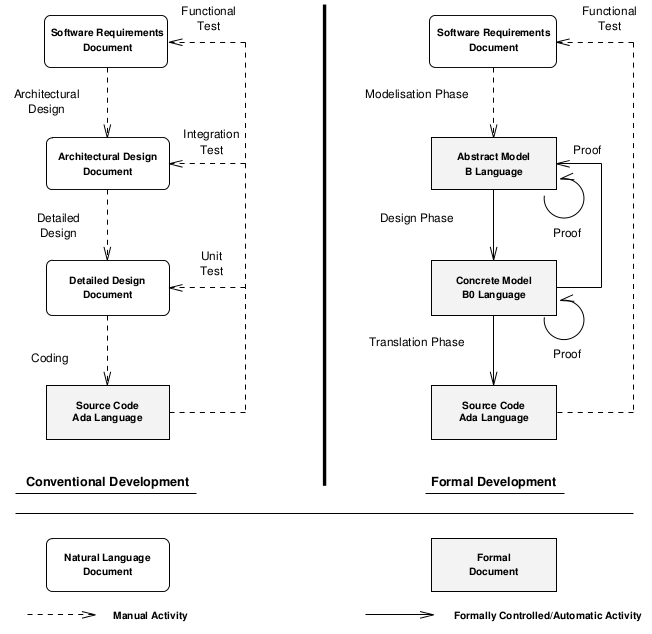
\includegraphics[scale=0.33]{ressources/formal_dev.png}
\end{figure}
\end{frame}

%
% Plan
%
\frame{\tableofcontents}

\section{Modélisation formelle}
\begin{frame}
\frametitle{Les machines abstraites}
\framesubtitle{Un exemple}

\end{frame}

\section{L'implémentation}


\begin{frame}
\frametitle{Questions ?}

\end{frame}

\end{document}